% 本章使用的 BibTeX 键：faugeras1993。

\section{相机模型与对极几何}
\label{sec:camera-model-epipolar-geometry}

本节简要回顾本文所需的透视投影数学背景，更多细节可参见
\citet{faugeras1993}.

\subsection{相机模型}
\label{sec:camera-model}

针孔相机由其光心 $C$ 和成像平面（图像平面）$\mathcal{R}$ 建模。三维点
$W$ 投影到图像点 $M$，后者是 $\mathcal{R}$ 与经过 $C$ 和 $W$ 的直线的交点。经过
$C$ 且垂直于 $\mathcal{R}$ 的直线称为光轴，它与 $\mathcal{R}$ 的交点称为主点。
$C$ 与 $\mathcal{R}$ 之间的距离是焦距。

设 $w=[x\;y\;z]^{\mathsf T}$ 是 $W$ 在任意固定世界参考系中的坐标，
$m=[u\;v]^{\mathsf T}$ 是 $M$ 在图像平面（像素）中的坐标。从三维坐标到二维坐标的
映射是透视投影，它在齐次坐标中表示为线性变换。令
$\tilde{m}=[u\;v\;1]^{\mathsf T}$ 和 $\tilde{w}=[x\;y\;z\;1]^{\mathsf T}$ 分别为
$M$ 和 $W$ 的齐次坐标，则透视变换由矩阵 $\widetilde{P}$ 给出：

\begin{equation}
  \tilde{m}\simeq \widetilde{P}\tilde{w},
  \label{eq:perspective-projection}
\end{equation}

其中，$\simeq$ 表示相差一个尺度因子时相等。因此，相机由其透视投影矩阵
（下文简称 PPM）$\widetilde{P}$ 建模。利用 QR 分解，该矩阵可分解为

\begin{equation}
  \widetilde{P}=A[R\mid t]
  \label{eq:ppm-factorization}
\end{equation}

矩阵 $A$ 仅依赖于内参数，其形式为

\begin{equation}
  A=
  \begin{bmatrix}
    \alpha_u & \gamma & u_0\\
    0 & \alpha_v & v_0\\
    0 & 0 & 1
  \end{bmatrix}
  \label{eq:intrinsic-matrix}
\end{equation}

其中，$\alpha_u=-f k_u$、$\alpha_v=-f k_v$ 分别是水平方向和垂直方向的像素焦距（$f$
为毫米单位的焦距，$k_u$ 和 $k_v$ 分别是沿 $u$ 轴和 $v$ 轴每毫米对应的有效像素数）；
$(u_0,v_0)$ 是主点坐标，即光轴与成像平面的交点；$\gamma$ 是描述 $u$ 轴和 $v$ 轴
不正交性的斜切因子。

相机的位置和姿态由 $3\times3$ 旋转矩阵 $R$ 以及平移向量 $t$（外参数）编码，
它们表示将相机参考系变换到世界参考系的刚体变换。

将 PPM 写为

\begin{equation}
  \widetilde{P}=
  \begin{bmatrix}
    q_1^{\mathsf T} & q_{14}\\
    q_2^{\mathsf T} & q_{24}\\
    q_3^{\mathsf T} & q_{34}
  \end{bmatrix}
  =[Q\mid\tilde{q}]
  \label{eq:ppm-block-form}
\end{equation}

在笛卡尔坐标中，投影（式~\eqref{eq:perspective-projection}）可写为

\begin{equation}
  \begin{cases}
    \displaystyle u=\frac{q_1^{\mathsf T}w+q_{14}}{q_3^{\mathsf T}w+q_{34}},\\[1.2ex]
    \displaystyle v=\frac{q_2^{\mathsf T}w+q_{24}}{q_3^{\mathsf T}w+q_{34}}
  \end{cases}
  \label{eq:cartesian-projection}
\end{equation}

焦平面是一个与成像平面平行且经过光心 $C$ 的平面。光心 $C$ 的坐标 $c$ 为

\begin{equation}
  c=-Q^{-1}\tilde{q}
  \label{eq:camera-center}
\end{equation}

因此，$\widetilde{P}$ 可以写成

\begin{equation}
  \widetilde{P}=[Q\mid-Qc]
  \label{eq:ppm-camera-center}
\end{equation}

与图像点 $M$ 对应的光线是直线 $MC$，即三维点集合
$\{w:\tilde{m}\simeq\widetilde{P}\tilde{w}\}$。其参数形式为

\begin{equation}
  w=c+\lambda Q^{-1}\tilde{m},\qquad \lambda\in\mathbb{R}
  \label{eq:optical-ray}
\end{equation}

\subsection{对极几何}
\label{sec:epipolar-geometry}

考虑由两个针孔相机构成的双目系统（图~\ref{fig:epipolar-geometry}）。设 $C_1$ 和
$C_2$ 分别为左、右相机的光心。三维点 $W$ 投影到两个成像平面上的点 $M_1$ 和
$M_2$，二者构成一个共轭点对。给定左图像平面中的点 $M_1$，其在右图像中的共轭点
被约束在一条称为（关于 $M_1$ 的）对极线的直线上。由于 $M_1$ 可能是其光线上任意点的投影，
这条对极线就是将 $M_1$ 的光线经 $C_2$ 投影所得的直线。一个图像平面中的所有对极线
都经过同一个公共点（分别为 $E_1$ 和 $E_2$），该点称为极点，它是另一相机光心的投影。

\begin{figure}[tb]
  \centering
  \IfFileExists{figures/fig1.png}{%
    \includegraphics[width=0.58\linewidth]{figures/fig1.png}%
  }{%
    \IfFileExists{task1/figures/fig1.png}{%
      \includegraphics[width=0.58\linewidth]{task1/figures/fig1.png}%
    }{%
      \fbox{\parbox[c][3.0cm][c]{0.72\linewidth}{\centering 图 1 原图待提取\\\small 路径：figures/fig1.png}}%
    }%
  }
  \caption{对极几何。第一相机的极点 $E_1$ 是第二相机光心 $C_2$ 的投影，反之亦然。}
  \label{fig:epipolar-geometry}
\end{figure}

当 $C_1$ 位于右相机的焦平面内时，右侧极点位于无穷远处，因而右图像中的对极线形成
一束平行直线。一个非常特殊的情形是两个极点都位于无穷远处；当直线 $C_1C_2$
（基线）同时包含在两个焦平面内，即成像平面平行于基线时，就会出现这一情形。此时，
两个图像中的对极线都形成平行直线束。

任意一对图像都可以经过变换，使各自图像中的对极线变为平行且水平的直线。这个过程
称为立体校正。
